\chapter{Ising model and complexity theory}


Quantum annealers are essentially different from classical computers. For one, they don't
execute programs written as a sequence of instructions in their memory. Instead, they are
single--purpose devices capable (in principle) of solving a specific optimization problem.
Namely, annealers are designed to find the lowest energy configuration (called \emph{ground state})
of the Ising spin--glass model, which we introduce in this chapter.

The potential usefulness of quantum annealers stems from the fact that the optimization problem they
are supposed to solve is hard for classical computers. But what does it formally mean for a problem
to be hard? To answer this question, we will need a brief recap of complexity theory, which is a
second point of this chapter.

Finding a ground state of the Ising spin--glass model may be hard for classical computers, but
there exists a plethora of heuristic, classical algorithms capable of finding solutions that are at
least ``good enough''. We conclude this chapter by listing and describing some of them.
These algorithms will serve as a baseline for comparison with quantum annealing and a recent
tensor network--based approach discussed later in the thesis.

\section{Ising model}

The Ising spin--glass model was introduced in 1920 by Wilhelm Lenz \cite{lenz} as a description of
ferromagnetism in solids but is named after his student Ernst Ising, who studied and solved it in
the one-dimensional case \cite{ising}. For purposes of this thesis, however, we will forget about
the physical interpretation of the model, treating it as merely as a description of a particular
optimization problem.

Consider a simple\footnote{That is, one that does not contain duplicate edges or loops.}, undirected
graph $G = (V, E)$ with $N$ nodes labeled by consecutive natural numbers.  With each node, $i \in V$
we associate a dichotomous spin variable $s_i \in \{-1, 1\}$. To each edge $\{i, j\} \in E$, we
assign an interaction strength $J_{ij}$ and to each node $i \in V$ we assign a local magnetic field
$h_i$. Here, all $J_{ij}$ and $h_i$ are real numbers. For such a system, one can define the
following energy function (Hamiltonian)
\begin{equation}
\label{eq:ising-hamiltonian}
H(\mathbf{s}) = \sum_{\langle i, j \rangle} J_{ij} s_i s_j +  \sum_{i=1}^N h_i s_i,
\end{equation}
where $\mathbf{s} = (s_i, \ldots, s_N)$ and the first sum runs over all edges in $E$\footnote{In the
literature, the Ising Hamiltonian \eqref{eq:ising-hamiltonian} is often negated. However, the
definition provided here is consistent with the one used by D-Wave, and thus more suitable for use
in this thesis}.

For fixed model coefficients, one is typically interested in finding its \emph{ground state}, a
configuration $\mathbf{s}$ that minimizes $H$. More generally, it might be desirable to search for
$k \ll 2^N$ configurations with the lowest energy, a so-called \emph{low--energy spectrum}.

\begin{figure}[H]
    \centering
    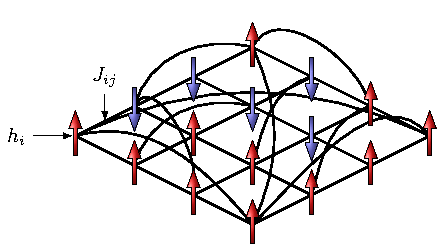
\includegraphics{figures/spins.pdf}
    \caption{Symbolic representation of Ising spin--glass defined on the graph with $N=16$ nodes. Here, $h_i$ is a real number associated with $i$-th node, and $J_{ij}$ denotes coupling strength associated with an edge between $i$-th and $j$-th node. The configuration of each spin is marked by a red arrow pointing upwards (+1) or a blue arrow pointing downwards (-1).}
    \label{fig:my_label}
\end{figure}

\begin{example}
Consider an Ising model instance with 3 spins given by the Hamiltonian $H$:
\begin{equation}
H(s_1, s_2, s_3) = s_1 - s_2 +2s_3 - 2s_2s_3 + 3s_1s_2
\end{equation}
This instance has 8 possible states:

\begin{table}[h]
    \begin{center}
        \begin{tabular}{|c|c||c|c|}
        \hline
        $\mathbf{s}=(s_1, s_2, s_3)$ &
        $H(\mathbf{s})$ &
        $\mathbf{s}=(s_1, s_2, s_3)$ &
        $H(\mathbf{s})$\\\hline
        (-1, -1, -1) & -1 & (1, -1, -1) & -5\\ \hline
        (-1, -1, 1) & 7 & (1, -1, 1) & 3 \\ \hline
        (-1, 1, -1) & -5 & (1, 1, -1) & 3 \\ \hline
        (-1, 1, 1) & -5 & (1, 1, 1) & 3\\ \hline
        \end{tabular}
    \end{center}
\end{table}
Observe that the lowest attainable energy is -5 and there are 3 states with this energy (we call
this situation a \emph{degeneracy}). Hence, all the configurations $(-1, 1, -1), (-1, 1, 1), (1,
-1, -1)$ are ground states. For this instance, a low energy spectrum of size $k=5$ comprises all
ground states, the $(-1, -1, -1)$ state with $H(-1, -1, -1) = -1$ and any of the states with
$H(\mathbf{s})=3$.
\end{example}

Despite the simple formulation, the problem of finding a ground state of Ising spin--glass is
computationally hard \cite{barahoma}. Before expanding on this idea, let us first introduce the
hierarchy of complexity classes.

\section{Algorithms and complexity}


Solving the computational problem requires a suitable \emph{algorithm}, a description of steps to be
performed by a computer to obtain a solution. It is hardly surprising that some problems might be
solved in more than one way, i.e. there might exist different algorithms performing essentially the
same task. Different algorithms solving the same problems might vastly differ in their demand on
various resources, like memory or time needed to execute them. In practice, execution time (and
usage of other resources) of a given algorithm might also vary between its implementations,
depending on factors like programming language or libraries used and the hardware it is executed on.
Therefore, measuring execution time is not that useful in characterizing the algorithm's
performance.  Instead, it is more useful to characterize algorithms based on how their execution
time scales (asymptotically) with increasing problem size\cite{arora}. For instance, given an
algorithm with execution time roughly proportional to the input size $N$, one might suspect that for
problem instances large enough, it will perform better than the one with execution time proportional
to $N^{2}$. This characteristic, known as computational complexity\footnote{Note that here we focus
only on \emph{time complexity}, but other notions like memory complexity can be defined similarly},
can be formalized by a big-$O$ notation (see appendix for more detailed description). Using this
notation, the algorithms from the above example would be classified as $O(N)$ and, $O(N^{2})$
respectively.

\section{Complexity classes}
Although there might exist multiple algorithms for solving a given computational problem, one might
consider the minimal time complexity required to do so. More generally, one might group
computational problems based on their demand on resources. In this view, sets of similar problems
are called \emph{complexity classes} \cite{arora}. The definition of some complexity classes might
also be restricted to specific types of problems. For instance, one might consider only decision
problems \cite{arora}, i.e. problems to which the answer is yes or no.

One of the fundamental complexity classes is \textbf{P}, a class of decision problems solvable in polynomial time on a deterministic Turing Machine  \cite{arora}. Another class, \textbf{NP}, comprises all decision problems whose solution can be verified in polynomial time using a deterministic Turing Machine \cite{arora}.
One can immediately see that \textbf{P} $\subset$ \textbf{NP}. Indeed, if a problem is solvable in polynomial time, then it is also trivially verifiable in polynomial time. However, it is not immediately obvious if the inclusion is strict, and whether \textbf{P} $\ne$ \textbf{NP} is one of the most important, yet unsolved problems in theoretical computer science \cite{fortnow}.
The class of \textbf{NP--hard} problems comprises all the problems that are at least as hard as
every problem in \textbf{NP}. More formally, given decision problem P is \textbf{NP--hard} if and
only if solving every problem in \textbf{NP} can be reduced to solving P a polynomial number of times
\cite{arora}. A particular subclass of \textbf{NP--hard} problems, \textbf{NP--complete}, is an
intersection of \textbf{NP} and \textbf{NP--hard} \cite{arora}. Figure \ref{fig:complexity} shows
the relationship between the discussed complexity classes, both under assumptions \textbf{P} =
\textbf{NP} and \textbf{P} $\ne$ \textbf{NP}.

Problems in the complexity class \textbf{P} are often considered tractable, or efficiently solvable,
whereas problems not in \textbf{P} are perceived as hard and computationally demanding, a statement
known as the Cobham's thesis \cite{cobham, arora}. At first, one might find it strange and
unintuitive. After all, a decision problem for which the best known algorithm runs in $O(N^{10^5})$
time is definitely in  \textbf{P}, but can hardly be called efficiently solvable. However, such
large polynomial complexities are rarely encountered in practice. Furthermore, even in such cases,
it is not uncommon that a better algorithm (e.g. with complexity $O(N^5)$) is found shortly after
the original one is discovered \cite{arora}.

\begin{figure}
    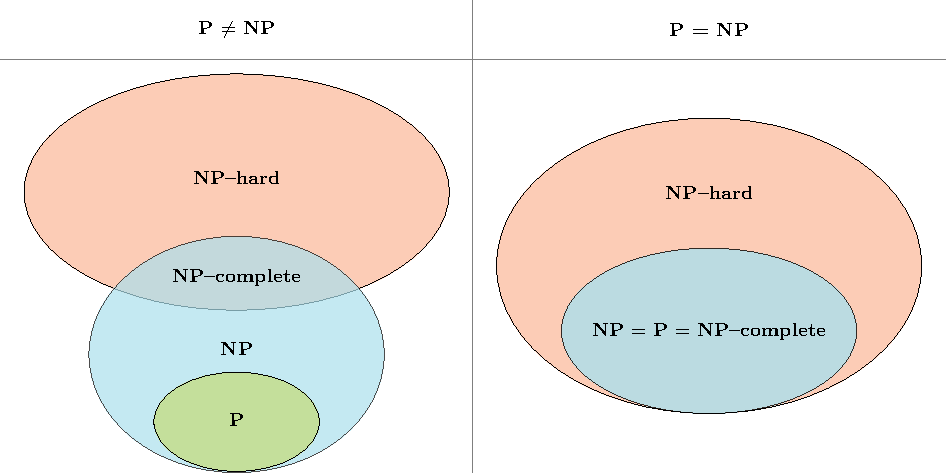
\includegraphics[width=\textwidth]{figures/complexity_new.pdf}
    \caption{Hierarchy of basic complexity classes. Under the assumption of $\textbf{P} \ne \textbf{NP}$ (left), the hierarchy is richer and there exist problems in \textbf{NP}  that are not \textbf{NP}--complete. Under the opposite assumption (right), the hierarchy collapses. Notice that in both cases there exist \textbf{NP}--hard problems that are not in \textbf{NP}
    }
    \label{fig:complexity}
\end{figure}



\section{Ising model and complexity}

Thus far, we only discussed classes of decision problems. How do they relate to the problem of
finding a ground state of the Ising model? Suppose we are given an Ising model instance with
hamiltonian $H$ and let $x \in \RR$ be some fixed number. Consider the problem of deciding whether
there exists $\mathbf{s}$ such that $H(\mathbf{s}) \le x$. We will call this problem a
\emph{decision version of the Ising problem}.

If we can minimize $H$, we can also solve the decision problem by simply finding a ground state and
checking if its energy exceeds threshold $x$. On the other hand, the sole capability of solving the
decision version of a problem does not give us an algorithm for solving an original optimization
problem. Therefore, one can see that the optimization problem is at least as hard as the
corresponding decision problem. Of course, the same reasoning applies for other optimization
problems. Hence, if the decision version of an optimization problem is \textbf{NP--hard},
the optimization problem is sometimes also called \textbf{NP--hard}, even if it slightly abuses the
notation. For simplifying the vocabulary, in what follows we will use this slightly
incorrect but more concise convention.

One can immediately see, that the state space of the Ising model with $N$ spins comprises $2^{N}$
different configurations. It might be tempting to reason that a problem with such an enormous number
of possible solutions must be \textbf{NP--hard}. While this is indeed the case, the size of the
solution space itself is not enough to reason about the problem's hardness\footnote{For instance,
the number of possible spanning trees in the complete graph of $N$ vertices is $N^{(N-2)}$, yet the
minimum spanning tree problem is solvable in polynomial time via several algorithms \cite{clrs}}.
It was shown that finding a ground state of the Ising spin--glass in the case of three-dimensional
lattices, as well as for some planar graphs,  is \textbf{NP--hard} \cite{barahoma}. The decision
version of the problem is \textbf{NP--complete}. Multiple known \textbf{NP--hard} problems, such as
Travelling Salesman Problem or Hamiltonian Cycles Problem, are reducible to finding the ground state of Ising spin-glass \cite{lucas}.

\section{Algorithms for solving Ising model}

\begin{figure}
    \centering
    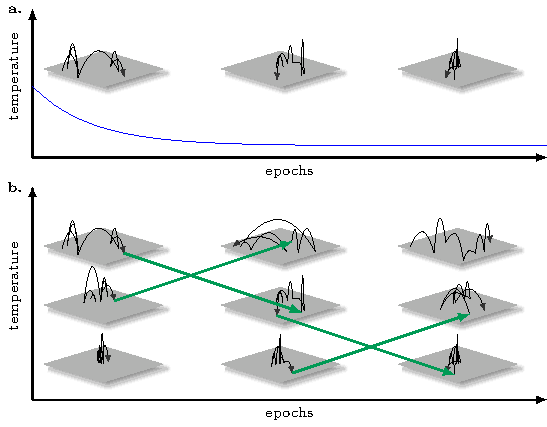
\includegraphics[width=\textwidth]{figures/pt_and_sa.pdf}
    \caption{Schematic representation of simulated annealing \textbf{(a)} and parallel tempering \textbf{(b)} algorithms. In simulated annealing, a single copy of the system is simulated. The temperature of the system is decreasing with each epoch, thus reducing movement through the state space. In parallel tempering, several copies (replicas) of the system are simulated, each with a fixed temperature. Hotter replicas move through the state space rapidly and less predictably, while colder replicas move conservatively. Between epochs, replicas can exchange states, which helps avoid being stuck at local minima. Exchanging replicas can also be viewed as reseeding of the colder replicas by randomized solutions provided by hotter replicas.}
    \label{fig:sa}
\end{figure}


As is the case with many \textbf{NP--hard} optimization problems, there are many heuristic
approaches for solving the Ising model. One family of such algorithms relies on the Metropolis-Hastings
\cite{beichl} algorithm for sampling from the underlying Boltzmann distribution. In simulated annealing
\cite{cook, isakov}, one lowers the temperature over time. Thus, the chance of accepting a locally
worse solution is greater at the start of the algorithm and decreases with each iteration, which
helps avoid getting stuck in a local minimum. In another approach from the same family,
\emph{parallel tempering}, one simulates several replicas of the system, each of them in a different
temperature. Neighboring replicas are allowed to exchange states, with exchange probability
depending on their energy and temperature difference \cite{swendsen}. Replicas with higher
temperatures explore state space rapidly (thus reseeding the algorithm), while ones with lower
temperatures refine the best solutions found so far. Various modifications of the aforementioned
algorithms exist. For instance, one could employ isoenergetic cluster moves \cite{zhu} or adaptive
choosing the number of sweeps performed between replica exchanges \cite{bittner}. Population
annealing is another Monte Carlo method, sharing similarities with simulated annealing and parallel
tempering \cite{wang}. Other approaches for solving Ising spin--glasses include methods involving
branch--and--bound framework \cite{rendl}, its chordal extensions \cite{baccari} or methods based on
simulating dynamical systems \cite{sheldon}.
%%% Local Variables:
%%% mode: latex
%%% TeX-master: "../main"
%%% End:
